\section{Sistemas Embarcados}

Para realização do projeto é necessário um sistema embarcado para controle dos sensores e atuadores, e intermédio de interface com o usuário.

Um sistema embarcado é um sistema de computador com uma função dedicada dentro de um sistema mecânico ou elétrico maior e geralmente com restrições de computação em tempo real. E é incorporado como parte de um dispositivo completo, muitas vezes incluindo peças mecânicas e de hardware. Sistemas embarcados controlam muitos dispositivos em uso comum hoje em dia. Noventa e oito por cento de todos os microprocessadores são fabricados como componentes de sistemas embarcados\cite{heath2003}.[6]

Exemplos de propriedades de computadores embarcados típicos quando comparados com os correspondentes de uso geral, são de baixo consumo de energia, tamanho pequeno, faixas operacionais robustas e baixo custo por unidade. Isso ocorre com o preço de recursos de processamento limitados, o que os torna significativamente mais difíceis de programar e interagir. No entanto, construindo mecanismos de inteligência sobre o hardware, aproveitando os possíveis sensores existentes e a existência de uma rede de unidades embarcadas, é possível gerenciar os recursos disponíveis de forma otimizada nos níveis de unidade e rede, bem como fornecer funções aumentadas, muito além aqueles disponíveis. Por exemplo, técnicas inteligentes podem ser projetadas para gerenciar o consumo de energia de sistemas embarcados\cite{heath2003}\cite{michael2007}.[6][7]

Os sistemas embarcados modernos são frequentemente baseados em microcontroladores (isto é, CPUs com memória integrada ou interfaces periféricas), mas microprocessadores comuns (usando chips externos para circuitos de memória e periféricos) também são muito utilizados, especialmente em sistemas mais complexos. Em ambos os casos, o processador a ser utilizado  pode ser de tipos variados, desde fins gerais até aqueles especializados em certas classes de cálculos, ou até mesmo customizados para a aplicação em questão\cite{heath2003}\cite{michael2007}. [6][7]

Como o sistema embarcado é dedicado a tarefas específicas, os engenheiros de projeto podem otimizá-lo para reduzir o tamanho e o custo do produto e aumentar a confiabilidade e o desempenho. Alguns sistemas embarcados são produzidos em massa, beneficiando-se de economias de escala\cite{michael2007}.[7]

\section{Medição do Nível da Água}

Os três tipos básicos de medição de nível são:
• direto
• indireto
• descontínuo
A medição direta pode ser feita medido-se diretamente a distância entre o nível do produto e um referencial previamente definido. Neste tipo de medição podemos utilizar a observação visual, como por exemplo, réguas, gabaritos, visores de nível, bóia ou flutuador, ou até mesmo através da reflexão de ondas ultra-sônicas pela superfície do produto\cite{cassiolato2010}.[8]

Na medição indireta, o nível é medido indiretamente em função de grandezas físicas a ele relacionadas, como por exemplo, pressão (manômetros de tubo em U, níveis de borbulhador, níveis de diafragma, células de pressão diferencial,etc), empuxo (níveis de deslocador) e propriedades elétricas(níveis capacitivos, detector de nível condutivo, níveis radioativos, níveis ultra-sônicos, detector de nível de lâminas vibrantes,etc)\cite{cassiolato2010}.[8]

Na medição descontinua, tem-se apenas a indicação apenas quando o nível atinge certos pontos especificados, como por exemplo, condições de alarmes de nível alto ou baixo\cite{cassiolato2010}.[8]

\section{Optoacopladores}

São dispositivos de proteção em circuitos eletrônicos que precisam trabalhar com diferentes tensões. No projeto da estufa eles serão utilizados para conectar a Raspberry a dispositivos que trabalham com tensão diferente de 3.3V, que é a tensão dos pinos GPIO, e para evitar uma sobrecarga de corrente nela.\cite{vishay}[3]

\section{Relé}

Os relés basicamente são dispositivos elétricos que tem como função produzir modificações súbitas, porém predeterminadas em um ou mais circuitos elétricos de saída. O relé tem um circuito de comando, que no momento em que é alimentado por uma corrente, aciona um eletroímã que faz a mudança de posição de outro par de contatores, que estão ligados a um circuito ou comando secundário. Resumidamente podemos dizer que todo relé se configura como um contato que abre e fecha de acordo com algum determinado fator ou configuração. Alguns relés são bem pequenos e fáceis de serem manipulados, testados e trocados, justamente por existir vários tipos de construções mecânicas para relés\cite{braga2012}. [4]

O relé é um componente eletromecânico, ou seja, ele conta com uma parte mecânica de contato e o acionamento ocorre através da corrente elétrica em uma bobina. Na imagem abaixo é possível visualizar todos os componentes de um relé eletromecânico\cite{braga2012}. [4]

\begin{figure}[H]
	\centering
	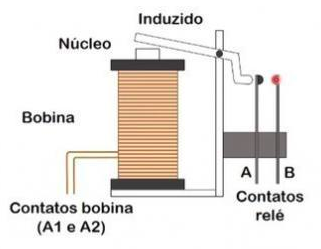
\includegraphics[width=5cm]{figuras/rele.png}
	\caption{Relé Internamente} \label{rele}
\end{figure}

\section{Conversor Analógico/Digital}

No mundo real as grandezas físicas raramente são de natureza elétrica. O primeiro passo para trazer esse mundo para o seu processador é o de transformar essas grandezas em sinais elétricos. Os equipamentos responsáveis por essa transformação são conhecidos por sensores ou transdutores. Esses transdutores estão em quase tudo ao nosso redor. São sensores de pressão, vazão, luz, temperatura, PH, etc. Todos esses transdutores transformam as grandezas físicas em sinais elétricos. Os sinais elétricos podem ser lineares e proporcionais à amplitude das grandezas medidas, ou então não lineares mas com curvas conhecidas, que podem ser compensadas de alguma maneira a posteriori\cite{braga2013}.[9]

Uma vez transformadas em sinais elétricos, a precisão das grandezas convertidas pelos transdutores fica limitada às características ou especificações desses transdutores. Sua natureza ainda é analógica e contínua no tempo. Para trazer essas grandezas para dentro do seu processador, será necessário realizar mais uma transformação do sinal analógico para digital, de forma que esse possa ser tratado e processado digitalmente. Essa transformação é realizada por um componente conhecido como Conversor A/D (Analógico/Digital)\cite{braga2013}.[9]
Um conversor A/D transforma um sinal analógico, contínuo no tempo, num sinal amostrado, discreto no tempo, quantizado dentro de um número finito de valores inteiros, determinado pela resolução característica do conversor em bits (8, 10, 12, 16 etc). Por exemplo, num conversor de 8 bits, o sinal de entrada é transformado em amostras com os valores entre 0 e 255\cite{braga2013}.[9]

O sinal a ser convertido por um conversor A/D dificilmente se acomoda diretamente à faixa de tensão de entrada do conversor. Ele precisa ser transformado adequadamente para isso. Em geral a tensão de entrada de um conversor A/D é definida como a tensão de alimentação do conversor (+ 5 ou 3,3 V, por exemplo). Para realizar essa adaptação muitas vezes é necessário realizar um condicionamento do sinal, tipicamente com auxílio de circuitos analógicos passivos ou ativos.

Após o condicionamento do sinal existe um elemento na entrada do conversor A/D que realiza uma amostragem periódica do sinal analógico e o mantém estável até que o conversor propriamente dito possa convertê-lo para um código digital. Trata-se de um circuito de Sample \& Hold. Um circuito ilustrativo de um S/H (Sample and Hold) pode ser visto na figura 2. A ilustração do efeito dessa amostragem pode ser vista na figura 3 \cite{braga2013}.[9]

\begin{figure}[H]
	\centering
	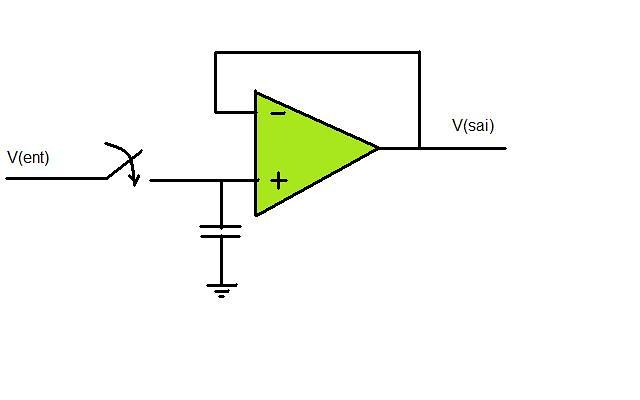
\includegraphics[width=9cm]{figuras/circuito_sample.jpg}
	\caption{Circuito Sample \& Hold simplificado} \label{circuito_sample}
\end{figure}

\begin{figure}[H]
	\centering
	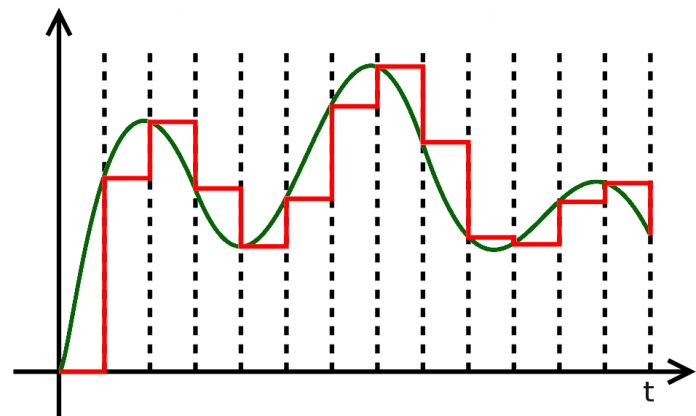
\includegraphics[width=9cm]{figuras/saida_sample.png}
	\caption{Saída de um circuito Sample \& Hold quando estimulada por um sinal contínuo} \label{saida_sample}
\end{figure}

